\documentclass{article}
\usepackage[UTF8]{ctex}
\usepackage{amsmath}
\usepackage{amsthm}
\usepackage{amssymb}
\usepackage[left=1.70cm, right=1.70cm, top=2.00cm, bottom=2.00cm]{geometry} %页边距

\usepackage{tikz}
\begin{document}
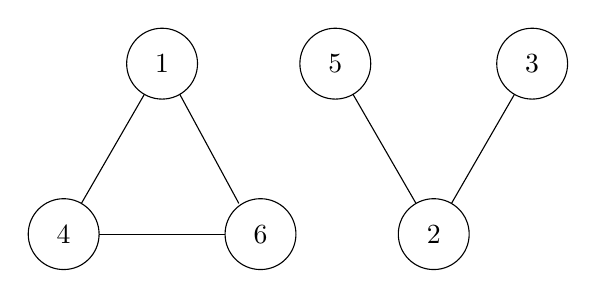
\begin{tikzpicture}
	\draw(0,0) circle [radius=0.45];
	\draw(2.5,0) circle [radius=0.45];
	\draw(1.25,2.165) circle [radius=0.45];
				\draw(0.45,0)--(2.05,0);
				\draw(0.225,0.3897)--(1.025,1.7753);
				\draw(1.475,1.7753)--(2.225,0.3897);
				\node[centered]at(0.0,0.0){4};
				\node[centered]at(2.5,0){6};
				\node[centered]at(1.25,2.165){1};
				
				\draw(4.7,0) circle [radius=0.45];
				\draw(3.45,2.165) circle [radius=0.45];
				\draw(5.95,2.165) circle [radius=0.45];
				\draw(4.475,0.3897)--(3.675,1.7753);
				\draw(4.925,0.3897)--(5.725,1.7753);
				\node[centered]at(4.7,0){2};
				\node[centered]at(3.45,2.165){5};
				\node[centered]at(5.95,2.165){3};
\end{tikzpicture}
\end{document}
